典型的USB设备的描述符一般由USB标准描述符和USB类描述符组成,或者由USB标准描述符和USB厂商特定描述符组成。任何一个USB设备都必须包含USB标准描述符,他提供了设备的基本信息和通信方式。为了简化USB设备的开发过程,通常会将具有相同的或者是相识的功能的设备归为一类,并指定相关的类规范,这样就能够保证只要按照同样的规范标准,即使是不同的厂商开发的USB设备也能够使用相同的驱动程序。针对不同类型的USB设备,USB-IF规定了相关的类描述符,他在标准描述符的基础上进一步说明了特定类型的设备共能以及相关的数据传输方式。但是USB-IF规定的设备类描述符并不能够覆盖所有的电子设备,对于没有相关的类描述符的USB接口,生产厂商需要利用自己提供的厂商特定功能的类描述符和设备命令对其通信特性做出说明,这些特定功能的描述符和命令的定义和操作完全取决于厂商,要想驱动此类设备就必须要参考厂商提供的这些专有命令。CP2102模块就属于这种没有相关的类描述符的设备,他不但支持USB的标准描述符和USB标准命令,还支持自己特定的描述符和命令,我们称这样的设备为非标准类型的USB设备。非标准的设备命令和描述符的结构和处理方式与标准设备命令和描述符是一样的,但是它只对特定的功能设备有效。
























驱动程序简单来说就是用来某个硬件的配置,使其能够完成固有功能的程序。驱动程序直接与硬件设备交互,其大多数的工作就是操作硬件相关寄存器。设备中的寄存器在系统掉电之后其内容会丢失,系统上电复位时其会复位到一个默认值,通常默认状态下的硬件是不能正常工作的,如中断使能被屏蔽,工作使能位也被屏蔽,还有一些决定硬件工作情况的关键控制寄存器也需要被重新配置。而这些工作都有赖于设备驱动完成。

换句话说,驱动代码具有系统特权级,除了其自身资源,对应硬件设备资源,其还对操作系统资源具有完全的访问权。
底层驱动很多时候用来定位硬件设计错误或者硬件芯片本身可能的问题,故底层驱动程序员必须对所要驱动的硬件设备有一个比较充分的了解,以及对与硬件交互的其他硬件或外界环境也需要有一个比较清楚的理解。









一个设备驱动在初始化过程中一方面完成硬件设备寄存器的配置,另一方面就是向

IO子系统注册驱动和设备,从而使得设备对用户可见。可以看到iosDrvInstall函数

参数为一系列函数地址,这些函数对应了为用户层提供的标准接口函数。一个驱动

无需提供以上所有函数的实现,对于无需实现的函数,直接传递 NULL指针即可。
iosDrvInstall函数基本实现即遍历drvTable数组,查

址对表项中各成员变量进行初始化,并将de_inuse设置为TRUE,最后返回该表项在

数组中的索引作为驱动号。设备初始化函数将使用该驱动号调用iosDevAdd将设备

添加到IO子系统中。此后用户就可以使用iosDevAdd函数调用时设置
询一个空闲表项,用传入的函数地

的设备节点名

对设备进行打开操作,打开后进行读写或控制

等其他操作,完成用户要求的特定功能。














驱动程序的编写是本次调试通道的核心部分,而驱动程序的编写与操作系统的关系密不可分。在VxWorks系统中,在控制器权转到设备驱动程序之前,用户的请求进行尽可能少的处理。VxWorks I/O系统的角色更像是一个转接开关,负责将用户请求转接到合适的驱动例程上。每一个驱动都能够处理原始的用户请求,到最合适它的设备上。另外,驱动程序开发者也可以利用高级别的库例程来实现基于字符设备或者块设备的标准协议。因此,VxWorks的I/O系统具有两方面的优点:一方面使用尽可能少的使用驱动相关代码就可以为绝大多数设备写成标准的驱动程序,另一方面驱动程序开发者可以在合适的地方使用非标准的程序自主的处理用户请求。
	USB口转串口设备作为非标准类型的USB设备,CP2102 USB/RS-232模块在连接到主机之后必须使用一个由开发者自己编写的设备驱动程序来驱动其正常工作,PC端的应用程序则无需任何更改,仍将其当做一个正常的串口设备来使用即可,但是本质上所有针对该串口发起的通信都是通过USB总线来传输的。而对于设备一方,收发的都是串行数据。	





串口作为计算机的一种标准接口,其硬件实现简单,且数据和控制信息是一位接一位的串行地传输下去的,比较适合于远距离传输,传输线路少。但是近年来由于其传输速度慢,扩展不方便,不支持热插拔等缺点,导致其逐渐的被各种设备所抛弃。而USB接口由于其速度快、连接灵活、支持即插即用等特点成为了设备标配接口。RS232和USB虽然都是属于串行接口, 但是他们的数据格式、通信协议以及信号电平定义和机械连接方式都完全不同\cite{何源2006USB},串口在某方面还是有RS-232串口无法替代的优势,尤其是USB口是一种主从式的接口,无法实现设备的双向控制,因此就催生出了USB口转串口的现实需求。









若需要相对一个圆形缓冲区的容量进行扩展,则需要对其中的数据进行搬移,这回对其应用造成相当的复杂性,因此使用环形缓冲区的应用应当是不需要调缓冲区的容量的。对于需要经常调整容量的缓冲区,使用链表来实现更为合适。

缓冲区当中需要考虑的关键问题是缓冲区的满和空的判断,因为缓冲区满或者是空都有可能出现读指针或者是写指针指向同一个位置。其检测方式基本有以下三种:
	
	\noindent \textbf{1. 使用一个空存储单元}\\
	在缓冲区中总是使一个存储单元保存为未使用的状态。即一个大小为N的缓冲区中最多只能够存入N-1个数据。如果读写指针指向同一个位置那么缓冲区即为空。如果写指针位于读指针的相邻后一个位置,那么缓冲区为满。这种策略的优点是简单、鲁棒;缺点是语义上实际可存储的数据量与缓冲区的容量不一致,测试缓冲区是否满需要做取余运算。
	
	\noindent \textbf{2. 使用数据计数}\\
	这种策略不适用显示的写指针,而总是保持着缓冲区内部的数据的计算。因此测试缓冲区是空是满非常简单;对性能的影响可以忽略。缺点是读写操作都需要修改这个存储数据计算,对于多线程访问缓冲区需要并发控制。
	
	\noindent \textbf{3. 使用镜像指示位}\\
	若缓冲区的长度是N,逻辑地址空间为0至N-1,那么规定N到2N-1为镜像逻辑地址空间。此时我们规定读写指针的地址空间为0至2N-1,其中低半部分对应于常规的逻辑地址空间,高半部分对应于镜像逻辑地址空间。当指针大于等于2N时,使其折返到ptr-2N的位置。使用一位表示写指针或者是读指针是否进入了虚拟的镜像存储区:置位表示进入,不置位表示没有进入。
	在读写指针的值相同的情况下,如果两者的指示位相同,说明缓冲区为空;如果两者的指示位不同,说明缓冲区为满。这种方法的优点是测试缓冲区满或空很简单,不需要做取余操作;读写线程能够分别设计专用算法策略,能够实现精致的并发控制。缺点是读写指针各需要额外的一位作为指示位。但是若缓冲区的长度为2的幂,那么我们不需要使用镜像指示位。此时如果读写指针的值相等,那么缓冲区即为空;若读写指针相差N,那么缓冲区为满,这可以使用条件表达式pWrite == (pRead \^ N) 来进行判断。 








本次设计的工作是一个VxWorks下的调试通道,由于设备上不存在串口,我们使用USB转RS232的方式来实现一个虚拟串口,设计的内容包括一个USB口转串口的驱动部分、基于USB口转串口驱动的应用层接口部分、windows下的调试信息分析界面部分。其中的重点在于本论文将要描述的基于VxWorks的调试通道部分,包括驱动部分和应用层的接口部分。
利用现有的CP2102模块能够轻松地完成USB/TTL的转换,开发者无需考虑总线枚举、数据收发与转换等工作,这些都由芯片自动完成。在windows和Linux下都有已经实现好了的基于CP2102的USB口转串口的驱动,但是在VxWorks下并没有这个驱动的实现,我们的调试通道的核心部分正是这个USB口转串口的驱动,因此我们需要在VxWorks中自己实现这个驱动程序。


\subsection{RS232与TTL}
	我们通常见到的串口有两种的物理标准,D型9针(对应于RS-232标准)插头和4针(对应于TTL标准)的杜邦头,4针的通常也会有第五根引脚--3.3V电源引脚。RS232电平标准用正负电压来表示逻辑状态,在RS-232标准中正电压是0,负电压是1。TTL电平标准使用高低电平来表示逻辑状态,TTL标准中低电平是0,高电平是1。使用TTL标准进行连接时,一般只会使用GND、RXD、TXD引脚,不会使用VCC或3.3V的电源线,避免与目标设备上的供电冲突。
	PL2303、CP2102芯片是USB转TTL串口的芯片,用USB来扩展串口(TTL)电平。	
 










\section{需求分析}
	根据项目上的实际需求,我们的调试通道需要满足一下的条件:
\begin{enumerate}
\item 为应用层实现接口部分,应用层只需要调用接口即可以实现调试信息的输出(无需实现串口的打开、关闭等操作),包括格式化和非格式化的信息。 

\item 实现一个特定的USB口转串口驱动,其需要具有一定的缓存能力,无论具体的设备是否连接上,都可以往这个设备中写入数据

\item 实现一个标准的USB口转串口的实现,与windows、Linux上的USB口转串口驱动的操作体验一致。

\item 实现一个windows客户端程序,能够接收自定义格式的输出和重定向的输出,并对自定义格式的输出进行正确的解析。
\end{enumerate}















	I/O 子系统在整个驱动层次中起着十分重要的作用,其对下管理着各种类型的设备驱动。换句话说,各种类型(包括网络设备)的设备都必须向I/O 子系统进行注册方可被内核访问。所以在I/O 子系统这一层次,内核维护着三个十分关键的数组用以对设备所属驱动、设备本身以及当前系统文件句柄进行管理。需要指出的是,VxWorks文件系统在内核驱动层次中实际上是作为块设备驱动层次中的一个中间层而存在的,其向I/O 子系统进行注册,而将底层块设备驱动置于自身的管理之下以提高数据访问的效率。在这些文件系统中,dosFs 和rawFs 是最常用的两种文件系统类型,在VxWorks早期版本就包含对这两种文件系统的支持。


















\section{VxWorks系统及驱动开发}

		
	VxWorks的基本构成部件由5个部分组成:板级支持包、wind内核、网络系统、文件子系统、IO系统。其结构如\autoref{fig:VxWorks系统结构}所示。
\begin{figure}[!h]
\centering
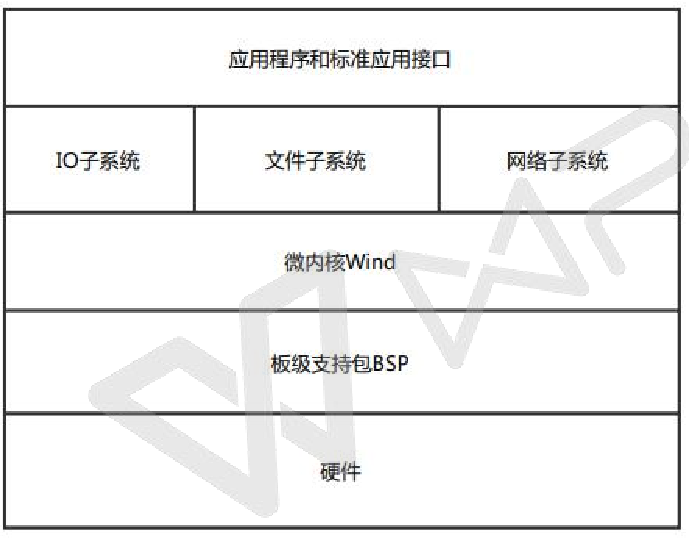
\includegraphics[width=.7\textwidth]{./graphics/VxWorks-sys-structure.pdf}
\caption{VxWorks系统结构}\label{fig:VxWorks系统结构}
\end{figure}

在本次的设计当中会使用到的部分包括VxWorks的wind内核部分和IO子系统部分,因此有必要介绍这两部分的相关内容。
	
\subsection{wind的任务调度}
	VxWorks采用微内核设计,其微内核被称为wind,其主要特点在于高效的任务管理(提供无限数量的的多任务,具有256个优先级,灵活快速的调度机制)、方便的任务间通信(提供多种信号量,网络通信以及共享内存等)、高度可裁剪(内核最小可以裁剪到8K)。由于VxWorks操作系统模块化非常好,模块间的耦合度非常低,每个模块对外提供都是单独的头文件,比如任务调度,其头文件为taskLib.h,任务通讯如果用的队列,那其头文件就是msgQLib.h,如果是定时器管理,那其头文件就是timerLib.h,因此也让程序移植提供了很大的便利性。	
	
	VxWorks下的任务即通用操作系统下所述的进程,是内核的基本运行单位,wind提供多任务环境,允许实时应用程序由单个或多个任务来构成,其中每个任务是程序的一个实例,每一个任务拥有独立的执行线程和一套自己的系统资源,同时由于在VxWorks中对内存进行统一编址,在任务间进行资源共享也十分方便,而任务间的通信机制可以使得得这些任务的行为同步、协调。
	wind将任务被分为256个优先级,0最高,255最低,任务在被创建时就会被指定一个优先级,在运行时也可以通过taskPrioritySet()函数重新设定优先级。VxWorks基于优先级来进行可抢占式的任务调度,对高优先级的情况进行优先响应。对于应用层任务,推荐使用100-250之间的优先级,驱动层任务可以使用51-99之间的优先级。
	
	VxWorks中任务的状态通常有四种,这四种状态可以通过相应的函数控制其相互转化如\autoref{fig:VxWorks状态转换图}。
\begin{itemize}
\item \textbf{就绪态:}任务正在等待CPU资源,该状态下以优先级为序排列任务。
\item \textbf{休眠态:}任务正在等待除CPU资源之外的其他资源,当竞争使用某个资源,而资源当前不可得,就进入这个状态。
\item \textbf{延迟态:}任务正在等待一定时间的延时。当调用taskDelay 函数让任务延迟一段固定的时间时,任务所处的状态,此时任务无资格竞争使用CPU。
\item \textbf{悬置态:}任务无法执行,主要是用于调试一种状态,这种状态仅影响任务的执行而不影响任务的转换。
\end{itemize}

\begin{figure}[!h]
\centering
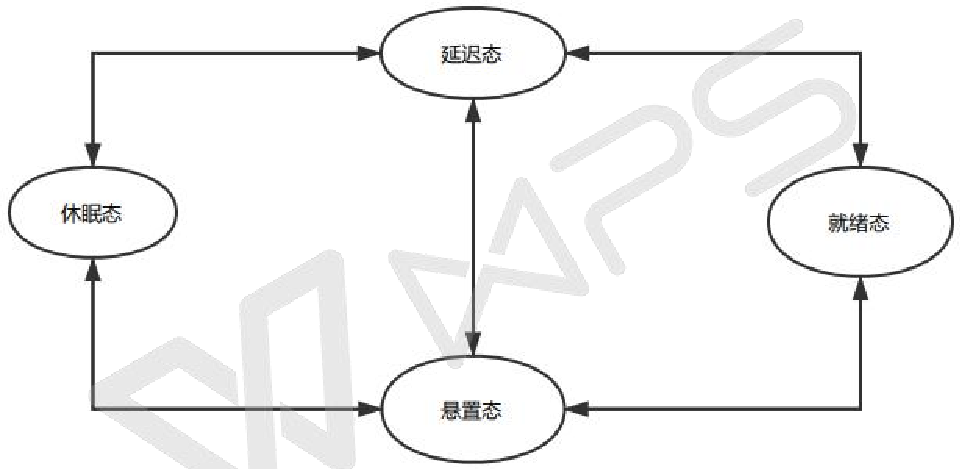
\includegraphics[width=.9\textwidth]{./graphics/vxworks-task-shift-diagram.pdf}
\caption{任务状态转换图}\label{fig:VxWorks状态转换图}
\end{figure}

	如\autoref{fig:wind任务调度}的wind内核任务调度框图展示了内核中构建了四种状态队列,通过TCB中任务状态的变化,由内核对其进行调度,并把就绪的任务加入到就绪队列等候CPU资源。
\begin{figure}[!h]
\centering
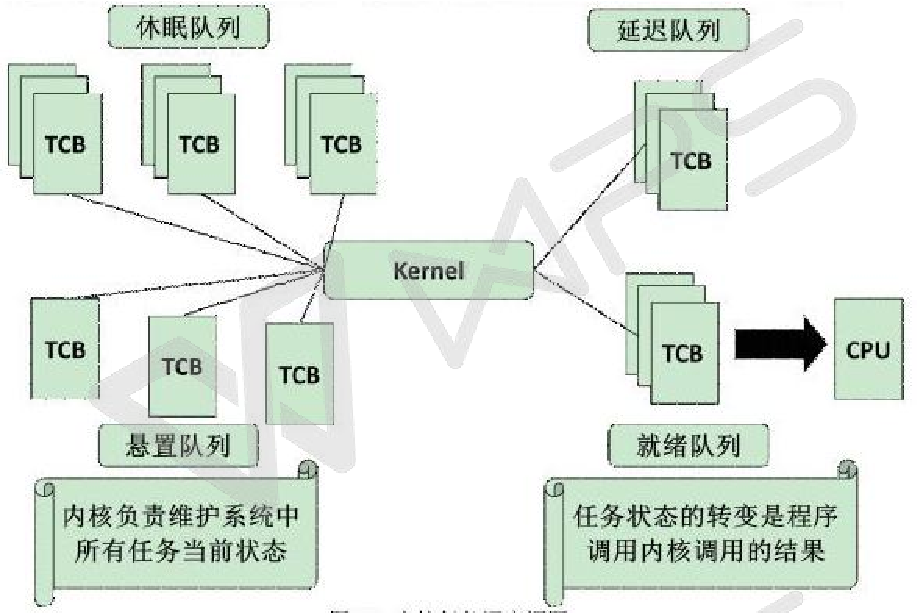
\includegraphics[width=.9\textwidth]{./graphics/vxworks-task-scheduling-diagram.pdf}
\caption{wind任务调度}\label{fig:wind任务调度}
\end{figure}\\
\textbf{任务调度机制:}

	wind将基于优先级的抢占调度作为缺省的调度策略,同级之间的任务依据时间片来进行CPU资源的分配。采用优先级抢占式调度算法符合实时系统的实际需求,紧急情况的出现需要及时的得到响应。这样用户对于需要尽快处理的任务就可以设置一个更高的优先级,保证其时间需求,而相对无关紧要的任务则设置一个较低的优先级。



\subsection{VxWorks设备驱动开发}
	
	根据设备的工作方式和数据的存储或者来源不同,可以将设备分为三大类:
\begin{itemize}
\item \hei{字符设备类型}

	字符设备以字节流的方式被访问,形同一个文件,但是字符设备无法移动文件偏移指针,只能顺序的访问数据。终端设备以及串口设备都属于字符设备类型。

\item \hei{块设备类型}

	块设备一般通过文件系统访问。而块设备的最多使用方式也是文件方式。块设备一般不能对单个字节进行访问,而是一个块的方式(如硬盘以一个扇区(512B)为单元进行访问)进行,允许同一数据的反复读取和写入。最典型的块设备就是硬盘,Flash 设备也是一种块设备。
	
\item \hei{网络设备类型}

	用于与网络上其他主机进行通信。其数据读取方式有些类似于字符设备,不可以对同一数据进行反复读写,只能顺序读写数据。且该类型设备区别于字符设备和块设备的一个很大的不同是,其不提供文件节点,任务要访问一个网络设备必须使用另一套网络套接字接口函数进行,与文件系统则完全不相关。网络设备底层数据传输上以块的方式进行,但是又不同于块设备中数据块的概念,网络设备中块的大小可以改变,但是有一个区间范围。
	
\end{itemize}

	以上只是设备类型的划分方式之一,事实上,按以上的划分标准,某些设备接口在某些情况下可以表现为任意以上三种形式之一,如 USB 接口,可以是一个字符设备,如 USB 串口;也可以是一个块设备,如 USB 内存卡;也可以是一个网络设备,如 USB 网络接口。

\section{USB口转串口驱动设计}

	对USB口转串口的设计通常可以采用两种方案,一种是以CY7C68013芯片为代表,自己从底层的固件开始,进行彻底而全面的系统开发,这种方案的成本和开发难度都很大,通常都不会使用这种方案。另外一个方案是采用类似于CP2102等专用的双向USB口转串口芯片来进行设计,这种方案简单实用,只需要对芯片的功能进行了解和应用即可,无需深入开发。因此我们在此会选择CP2102芯片来进行调试通道的设计。


\subsection{USB总线结构}
	USB(Universial Serial Bus,通用串行总线)是这十几年来应用在PC领域的最新型的接口技术,出现的契机是为了为了解决日益增加的PC外设与有限的主板插槽之间的矛盾,其实现是由一些PC大厂商(Microsoft、Intel等)定制出来的,自从1995年在Comdex上展出以来至今已广泛地被各个PC厂家所支持。目前已经在各类外部设备中都广泛的采用USB接口。USB接口标准目前有三种:USB1.1,USB2.0和USB3.0。USB接口应用如此的广泛是由其独特和实用的特性决定的。

\noindent USB规范规定了USB传输的四种方式,每种方式有各自的用途\cite{USB总线接口开发指南}:
\begin{itemize}
\item \hei{控制传输}:控制传输是每一个设备必须要具有的传输方式,也是四种传输方式中过程最复杂的部分,他使得主机能够从设备列出的范围中读取和选择配置和其他设置,也能够发送自定义请求来为任何目的而发送和接收数据,在配置和列举的过程中起到重要的作用。
\item \hei{批量传输}:批量传输是为了处理传输速率不是很关键的情况,一般用于打印机和扫描仪。
\item \hei{中断传输}:中断传输是为了那些要快速实现主机和设备的交互而准备的,比如适用于鼠标和键盘。
\item \hei{等时传输}:等时传输用于必须要按照一个常数传输数据的情况,比如一个需要被实时播放的视频/音频数据流。
\end{itemize}\\
所有的传输都是由事务组成,事务又由包组成,而包包含一个包识别器(PID)、CRC和其他的信息\cite{USB大全}。

	USB的体系结构如\autoref{fig:USB体系结构}所示
\begin{figure}[!h]
\centering
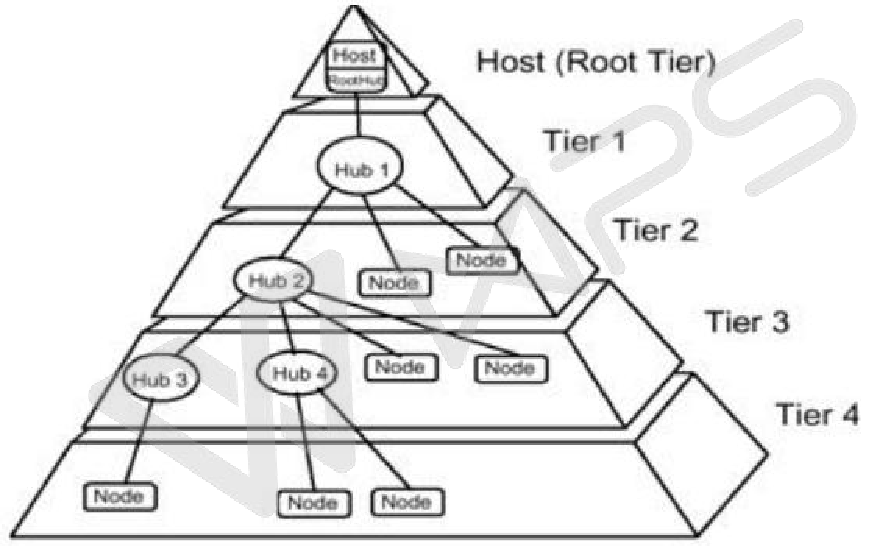
\includegraphics[width=1.0\textwidth]{./graphics/usb-structure.pdf}
\caption{USB总线拓扑结构}\label{fig:USB体系结构}
\end{figure}

	USB的物理层拓扑为星型结构,包括三个部分:USB主机(Host)、USB集线器(Hub)、USB设备(Device)。
	
\begin{enumerate}
\item \textbf{USB主机}

	USB的体系结构只允许系统中有一个主机,主计算机系统的USB接口称之为USB主控制器。主控制器可以是硬件、固件或软件的联合体,其控制着总线上所有USB设备和所有集线器的数据通信过程。所有的数据传输都是由USB的主机端发起的,而且如果USB主机嵌入在一个计算机系统中,在数据的传输过程中也不需要计算机的CPU参与传输工作。USB主机通常具有以下的功能:
	\begin{itemize}
	\item 检测USB设备的插拔动作(通过根集线器来实现)
	\item 管理 USB 主机和USB设备之间的控制流
	\item 管理USB主机和USB设备之间的数据流
	\item 收集USB主机的状态和USB设备的动作信息
	\end{itemize}
\item \textbf{USB集线器}
	
	根集线器是集成在主机系统当中的一个特殊集线器,他可以提供一个或者跟多的接入口。在即插即用的USB体系结构当中,集线器是一种很重要的设备。其极大的简化了USB的复杂性,而且以很低的价格和易用性提供了设备的健壮性,集线器的最大的连接能力是127。

\item \textbf{USB设备}

	USB设备是USB总线系统的重要组成部分,它们以从属的方式与USB主机进行通信,并受USB主机的控制。USB主机端提供的协议软件通过和USB设备通信获得设备的信息,并给设备提供驱动程序,相比USB主机而言,USB设备只能够被动的应答,按照USB主机的要求接受或者发送数据。USB设备通过以下的属性来完成主机的要求:
	\begin{itemize}
	\item \textbf{描述符}\\
	USB协议为USB设备定义了一套描述设备功能和属性的固定结构的描述符,通过这些描述符向USB主机汇报设备的各种属性,主机通过对这些描述符的访问对设备进行识别、配置并为其提供相应的客户端驱动程序。典型的描述符一般由USB标准描述符和USB类描述符,或者由USB标准描述符和USB厂商特定描述符组成。运行于USB协议栈上层的客户端驱动程序通过这些信息正确的访问设备并与其进行通信,以实现即插即用的目的。
	\item \textbf{类}\\
	USB协议支持许多的外围设备,为了正确的驱动这些设备,USB主机端要为这些设备提供符合USB协议的驱动程序,称为客户端驱动。同时为了避免客户端程序过多,协议通过归纳将设备划分为不同的设备类,把功能相近的设备归为一类,主机端只需要提供类驱动程序便可以驱动大多数的USB设备。	
	\item \textbf{功能(Function)/接口(Interface)}\\
	在USB协议中,Function被定义为具有某种能力的设备,即相当于传统的单一功能设备。随着USB设备应用的发展,物理上几种不同的Function可以组成一台设备,只要设备的接口具有某种独立的能力,就称为一个Function。Function是从功能角度来说的,从设备的角度来说,它又被称为Interface。
	\item \textbf{端点(Endpoint)}\\
	端点层的各个子模块是USB设备与USB主机逻辑上的数据传输的最基本单元,即最基本的通信点,因而端点层的每一个逻辑模块被称为端点(Endpoint)。每一个端点都关联一个相应的端点号和数据传输方向(IN/OUT)。具有相同端点号和不同传输方向的通信点表示不同的端点,端点0被USB规范保留用作设备枚举和配置过程中的数据传输端点,与端点0对应的管道是默认管道,设备的所有端点共享端点0。在一个USB系统当中,USB主机对特定设备功能的访问是通过使用不同的端点号,否则,USB主机将不能对相应的设备进行正确的访问。由于在系统运行时,不同的设备配置有着互斥性,因而在不同的配置描述中,端点号是可以重复的。
	\item \textbf{管道}\\
	设备端点与USB主机所形成的具有特定数据传输特性(如数据传输格式、传输带宽、传输方向等)的数据通道,被称为管道。管道的物理介质就是USB系统中的数据线。端点层的USB设备与USB主机之间的数据传输都是基于管道进行的。
	\item \textbf{设备地址}\\
	USB主机的客户端驱动程序通过描述符来区分不同的设备,而USB主机控制器通过设备地址来区分设备。设备地址共有7位,表示理论上系统可以同时连接127个USB设备,但是在实际中,由于USB总线带宽的限制,这么多设备不可能同时的工作。USB主机负责为USB系统中的设备分配不同的设备地址,用来表示哪个设备的同时还要指名设备的端点号,表示使用哪个管道。
	\end{itemize}	
	
\end{enumerate}

	一个主机和设备的连接需要一些列的层次和实体之间的交互,USB接口层在主机和设备间提供物理、信号包的关联,USB设备层表示USB系统程序实现对一个设备进行的总的USB操作,功能层适当匹配的客户服务程序层提供附加的功能给主机。设备和功能层当中各自有逻辑通信,但是实际的USB数据传输是通过USB总线接口层来实现的\cite{USB开发手册}\cite{圈圈教你玩USB}。

	
\section{调试通道总体设计}

	整个调试通道的设计包括两个部分,一个是应用层的接口的设计,一个USB口转串口的驱动程序的设计。整个系统的结构如\autoref{fig:debug-system-diagram}所示:
\begin{figure}[!h]
\centering
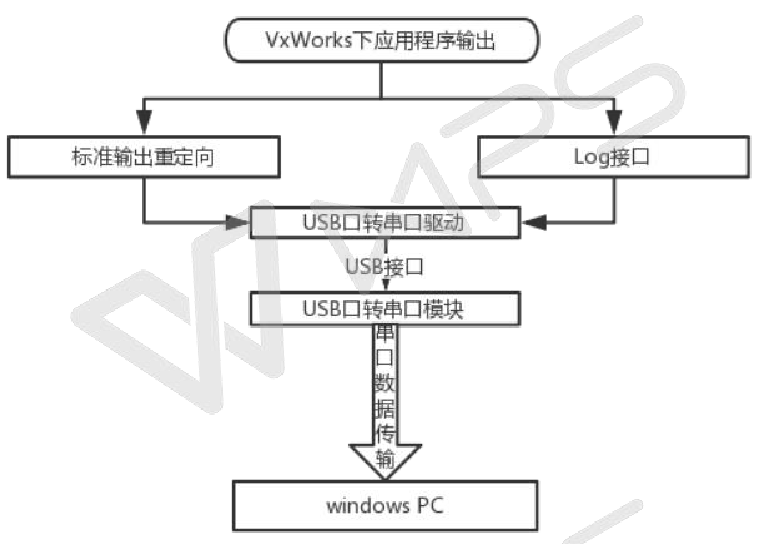
\includegraphics[width=.7\textwidth]{./graphics/debug-system-diagram.pdf}
\caption{调试通道整体结构图}\label{fig:debug-system-diagram}
\end{figure}































基于以上设备所需要实现的五大基本功能,我们可以得出凡是基于VxWorks内核调用的驱动程序不外乎以下的组成部分:

\begin{enumerate}
\item 设备驱动函数的注册函数。驱动开发人员必须要开发响应的函数将驱动程序的功能注册到设备驱动程序列表中,以便挂接到I/O系统。

\item 设备驱动的卸载函数。若系统不再使用设备,需要将其卸载掉,以节约系统资源

\item 设备的打开和关闭函数。这两个函数是相伴的,有打开操作就必须有关闭操作。

\item 设备的读写函数。主要完成设备的外设和CPU之间的数据交换。

\item 设备的控制函数。在使用设备的过程中,需要对设备的工作状态进行控制。

\item 中断服务函数(ISR)。响应外设的中断请求。
\end{enumerate}\\



\textsc{%此处集成开发环境应该将其删除,或者将移到其他的部分来简单的介绍。
\section{集成开发环境Tornado}

	Tornado是嵌入式实时领域里最新一代的开发调试环境,其系统结构如\autoref{fig:Tornado开发系统结构}所示。Tornado提供了高效明晰的图形化的实时应用开发平台,可以帮助轻松的完成程序的编辑、编译、调试、系统配置等工作。它包括一整套完整的面向嵌入式系统的开发和调试工具。Tornado采用的是主机—目标机的交叉开发模型,应用程序在主机的Windows环境下编译链接生成可执行文件,下载到目标机,通过主机上的目标服务器与目标机上的代理程序的通信完成对应用程序的调测、分析。这些工具包括C和C++远程级调试器、目标和工具管理、系统目标跟踪、内存使用分析和自动配置,所有工具都能够很方便的同时运行,很容易增加扩展和交互式开发。
\begin{figure}[!h]	
\centering
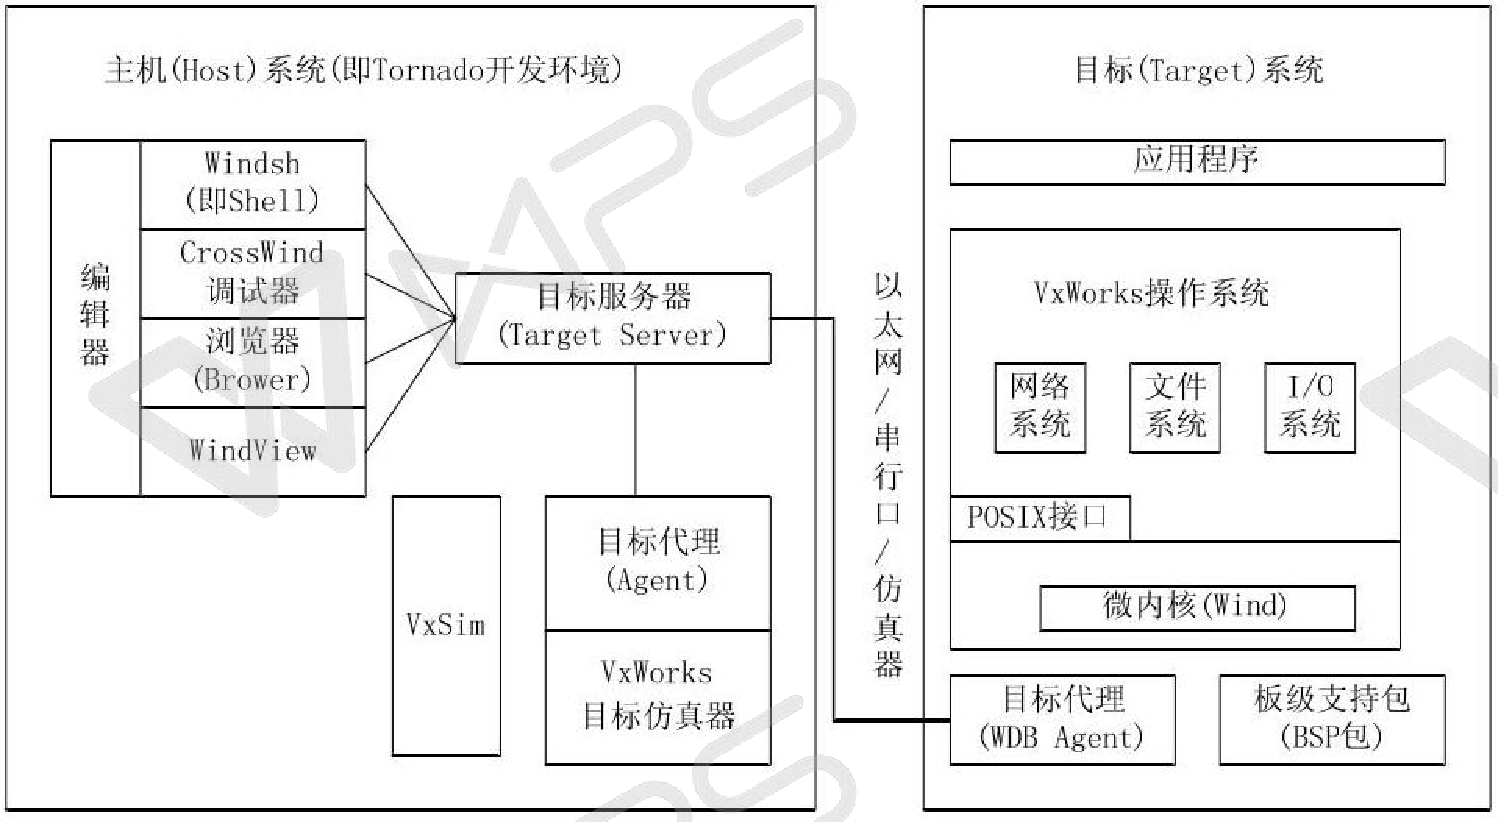
\includegraphics[width=1.0\textwidth]{./graphics/tornado-system-structure.pdf}
\caption{Tornado开发系统结构}\label{fig:Tornado开发系统结构}
\end{figure}
	
	典型的主机开发系统通常有比较大的RAM、硬盘空间、打印机以及其他外部设备,而典型的目标机系统只有仅能满足实时应用的资源,除此以外可能还有比较少量的用于测试和调试的额外资源。Tornado开发环境的基本优点是应用模块不需要链接到运行系统库。Tornado直接装载重定位的目标模块,通过每个模块里的符号表来动态解析外部符号的引用,解析符号表是由运行在目标机上的目标服务器来完成的。Tornado在开发过程中会把目标模块的大小减到最小,这样可以缩短开发周期。主机端驻留的shell和调试器也能够调用和测试独立的应用程序或者是完整的任务。

	Tornado是为开发VxWorks应用程序提供的集成开发环境,其中包含有工程管理软件,可以将用户自己的代码和VxWorks的核心有效的结合起来,可以按照用户的需要裁剪配置VxWorks内核;
Tornado开发系统包含有三个高度集成的部分:
\begin{itemize}
\item \hei{运行在宿主机和目标机上的强有力的交叉开发工具和实用程序;}
\item \hei{运行在目标机上的高性能、可裁剪的实时操作系统VxWorks;}
\item \hei{连接宿主机和目标机的多种通信方式,如以太网,串口线,ICE或ROM仿真器等。} 
\end{itemize}

Tornado主机集成开发环境中的主要工具为:
\begin{itemize}
\item \textbf{工程管理和配置工具:} 提供工作空间用于应用程序的组织和管理,可通过图形化的配置工具对VxWorks及其组件进行配置。
\item \textbf{交叉编译器:} 提供GNU和Diab两种交叉编译器和类库
\item \textbf{调试器:}提供图形界面的调试方式,可以通过编辑窗口的右键菜单来设置断点和查看变量;
\item \textbf{WindSh:} 一个驻留在主机端的命令行解释器,提供从主机端控制所有运行系统的接口
\item \textbf{CrossWind调试器:}一个远程源码级的调试器,该调试器控制窗口综合了GDB命令行接口和WindSh工具。
\item \textbf{浏览器:} 是一个系统对象的查看器,可以监视目标机的状态。
\item \textbf{WindView逻辑分析器:} 一个动态可视化工具,可以提供上下文切换的情况,事件和有关测量对象的信息。
\item \textbf{VxSim仿真器:} 用来模拟目标操作系统。
\end{itemize}

	位于主机上的目标服务器和位于目标机上的目标代理通过WDB(Wind Debug)协议完成主机和目标机之间的通信。二者无论采取哪种链接方式,都是基于WDB协议的。

	
		
	方便编程人员对系统进行分析、调试。同时基于应用程序的可移植性的考虑,VxWorks在其内核Wind中也支持 POSIX 1003.1b的规定和1003.1中有关基本系统调用的规定,包括:过程初始化、文件与目录、I/O 初始化、语言服务、目录处理;而且 VxWorks 还支持 POSIX 1003.1b的实时扩展,主要包括:异步 I/O、记数信号量、消息队列、信号、内存管理和调度控制等\cite{Wind2003VxWorks}。当然有些POSIX接口也有VxWorks下的实现重新实现版本,比如定时器、二进制信号量、消息队列等。VxWorks下专用的实现版本和POSIX兼容的实现版本在性能上有一些差异,POSIX的接口主要是为简化Linux下程序的移植而设立的。对于没有POSIX接口的部分则必须将程序修改为VxWorks下的接口,对于修改了的代码在VxWorks下运行可能会出现各种问题,本文为了给出一个事后对程序进行分析的方法,于是设计了这个基于VxWorks下的调试通道。



	串口因为其简单可靠、使用方便、开发成本较低等优点\cite{串口调试}。 数据传输是现代通讯过程中的一个重要环节,在数据的传输过程中,不仅仅要求数据传输的准确率要高,而且要求速度快,连接方便。传统的RS232串口通讯和并口通讯都存在传输速度低,扩展性性差、安装麻烦等缺点,而基于USB接口的数据传输系统能够较好的解决这些问题。目前USB接口以其传输速率高、即插即用、支持热插拔等优点,逐步成为PC机的标准接口。PC端的应用软件依然是针对串口进行编程,外设也是以串口为数据通道,但是从PC到外设的物理连接使用的却是USB总线,在上的数据通信也是USB数据格式。

	对于特性相异的设备要使用串行通信来连接时,必须保证双方所使用的的标准接口是一致的。一般的串口标准有RS-232、RS-485、TTL等。从通信的方向性来看,串口通信有单工、半双工和全双工三种方式。单工通常使用一根导线,通信只在一个方向进行,如监视器、打印机、电视机。半双工可以在两个方向上进行,但是方向切换时有时间延迟,如打印机。全双工可以在两个方向上运行,且时间的切换没有时间延迟,适用于那些不能有时间延迟的交互式应用,如远程监控等。






\begin{enumerate}
\item \hei{USB设备与主机系统的交互}

	MCU对USB芯片进行初始化:设置内部时钟,选择内部连接方式以及是否开通DMA传输等;设定设备的工作模式,并设备本设备的初始地址为0(USB规范指明当设备接入PC的时候都由初始为0的地址对主机进行响应,之后再由主机分配一个地址给USB设备,设备接收到分配地址命令后,再更改自己的地址,并一直通过这个地址完成后续的通信)。
	完成初始化工作之后,MCU将使能USB接口,主机系统将因此检测到一个新的USB接入而很快与设备进行握手,获取设备的基本信息,并完成一些列的对设备的配置,其过程为:
	\begin{enumerate}
	\item USB上电使能后,主机会向USB设备发送GET DEVICE DESCRIPTOR的命令,之后主机会收到设备发出的设备描述符,随即为设备分配一个空闲地址,并向设备发送SET ADDRESS的命令,这时设备通过地址0发送一个长度为0的数据包予以应答,然后根据主机的要求更改自身的地址,而且这以后的数据交换都将会通过这个新的地址来进行。
	\item 完成地址设备之后,主机将会发送GET CONFIGURATION DESCRIPTOR,USB规定当主机发出该命令符的时候,设备必须要同时返回配置所包含的所有接口和接口所包含的所有端点的描述符。
	\item 主机获取到USB设备的描述符、配置描述符并进行了地址设置之后,设备与主机的握手初步完成,之后会将该设备加入到设备列表当中。
	\end{enumerate}
	
	\item \hei{USB设备与驱动程序的交互}
	
USB设备的驱动与传统意义上的硬件驱动不完全相同,他并不与硬件直接通信,而是以创建和发送URB请求块的形式把命令传递给操作系统所提供的USB总线驱动程序,由总线驱动程序来完成与硬件的直接交互。和主机类似,驱动会首先创建和发送请求得到该设备的DEVICE DESCRIPTOR的URB,并将获取到的信息存储在专用的数据结构当中,接着驱动为了得到完整的设备配置,必须要通过总线驱动发送两次GET CONGFIGURATION DESCRIPTOR命令得到设备。获取设备的配置信息之后,驱动在启动设备之前还要发送SET CONFIGURATION、SET INTERFACE命令。通过以上的几个步骤便可以完成驱动与USB设备过程。	
\end{enumerate}



实时操作系统(Real Time Operation System,简称RTOS)是整个实时系统的核心。POSIX1003.1标准为RTOS下了一个简单的定义:RTOS是能够在有限的响应时间内为应用提供所要求级别服务的操作系统\cite{Renard20081003}。当外界事件或者是数据产生时,RTOS需要快速的进行处理,并且处理的结果又能够在规定的时间之内来控制生产过程或者对处理系统做出快速的响应,调度一切可利用的资源来完成实时任务。实时系统按照实时的效果可以分为软实时和硬实时,硬实时要求在规定的时间内必须完成操作,这是通过操作的在设计的时候就得到保证的;软实时只需要按照任务的优先级,尽可能快的完成任务即可。\\
一个实时操作系统的特征通常包括以下几点:
\begin{itemize}
\item \textbf{高精度计时系统}\\
	计时精度是影响实时性的一个重要因素,在实时系统当中,经常需要精确确定实时地操作某个设备或执行某个任务,或精确的计算一个时间函数。这些不仅仅依赖于一些硬件提供的时钟精度,也依赖于实时操作系统的高精度计时功能。
\item \textbf{多级中断机制}\\
	中断是实时操作系统当中的一个关键设施,是用于通知系统发生外部事件的常用机制。一个实时操作系统通常需要处理多种外部信息或事件,但处理的紧迫程度有轻重缓急之分。有的必须立即作出反应,有的则可以延后处理。因此,需要建立多级中断嵌套处理机制,以确保对紧迫程度较高的实时事件进行及时响应和处理。
\item \textbf{实时调度机制}\\
	实时操作系统不仅要及时响应实时事件中断,同时也要及时调度运行实时任务。但是,处理机调度并不能随心所欲的进行,因为涉及到两个进程之间的切换,只能在确保“安全切换”的时间点上进行,实时调度机制包括两个方面,一是在调度策略和算法上保证优先调度实时任务;二是建立更多“安全切换”时间点,保证及时调度实时任务。
\end{itemize}
本次所需完成的调试通道正是基于一个目前业界有名的实时操作系统VxWorks。






\subsection{VxWorks下驱动程序的开发}
	
	VxWorks作为一款嵌入式操作系统,为了屏蔽硬件的具体操作细节,为上层应用程序提供统一的接口,引入了设备驱动程序的概念。设备驱动程序是用来直接控制设备,以完成设备应有的操作。操作系统通过驱动程序来对设备进行操作,属于一种软件接口。这样,应用程序开发使用统一的软件接口,使得开发人员可以专注于应用程序的开发,不用考虑底层的物理设备。
	
	VxWorks操作系统下的驱动程序在其开发上有自身规范,且对于不同的设备的驱动程序开发也表现出较大的差异。嵌入式设备的硬件平台千差万别,厂商不可能遇见所有的设备并提供相应的驱动程序,因此要实现VxWorks的跨平台移植,用户必须要根据硬件平台开发驱动程序。所以,开发VxWorks操作系统下外围设备的驱动程序具有很大的实际应用价值。
		
	虽然VxWorks作为实时嵌入式系统有着无比强大的性能表现,但是就目前的现状来看,VxWorks操作系统的平台成本很高,因为VxWorks是一个专用系统,使用这个系统的单位或公司都是处于军事,航天等特殊行业当中,这使得他们的开发经验和资源不能够拿出来共享,导致VxWorks的参考资料比较少,没有成熟活跃的社区支持,且VxWorks并不是一个开源的系统,需要花不菲的价格进行购买和售后支持,这些都提高了VxWorks的应用的开发门槛,使得一般的开发人员不能够方便的接入到对其的应用研究当中,增加了开发难度。
	
	





	VxWorks系统主要如下几个组件,一般的应用程序也就用到如下几个模块:任务调度负责任务优先级,任务创建,任务删除等功能。任务通讯主要涉及队列管理,管道管理等。IO管理就是通用外设的输入输出管理。文件管理包含文件或者链接创建,修改,删除,检索等等。内存管理包含内存申请及内存释放。定时器管理就是定时器创建,定时器删除。网络通信包含套接字创建,udp/tcp通信,套接字删除,及配置管理。同步就是任务同步。互斥就是任务互斥,保护关键资源。
	
	在VxWorks操作系统的代码架构里面,一般写一个应用程序只需要涉及上面几个系统组件,由于VxWorks操作系统组件化非常好,这几个组件的耦合度非常低,每个组件对外提供都是单独的头文件,比如任务调度,其头文件为taskLib.h,任务通讯如果用的队列,那其头文件就是msgQLib.h,如果是定时器管理,那其头文件就是timerLib.h,因此也让程序移植提供了很大的便利性。有很多人认为,VxWorks跟Linux操作性的系统头文件差异化太大,因此移植难度成倍速增加,其实不然,就是由于VxWorks的高度组件化,让程序移植提供了很大的便利性。
	
	
	wind使用中断驱动和优先级的方式。它缩短了上下文转换的时间开销和中断的时间延迟。VxWorks中的任何例程都可以被启动为一个单独的任务,拥有它自己的上下文和堆栈,还有一些其他的任务机制可以使得任务挂起、继续、删除、延时或改变优先级。	
	
	
	板级支持包BSP(Board Support Package)作为VxWorks系统的主要组成部分,对各种板子的硬件功能提供了同一的软件接口,它包括硬件初始化、中断的产生和处理、硬件时钟和计时器管理、局域和总线内存地址映射、内存分配等。每一个板级支持包包括一个ROM启动(Boot ROM)或其他启动机制。

% appendix环境用于附录环境。即可以将附录置于appendix环境当中。如:
% \begin{appendix}
%  <content>
% \end{appendix}

% 直接使用\appendix 则表明后文均为附录。如:
% \appendix
%  <content> 
\appendix

% publications环境用于已经发表了的论文的页面,一般用于附录当中,使用上同enumerate环境
\begin{publications}
    \item 论文1
    \item 论文2
\end{publications}

\chapter{这是一个附录}\label{appendix:1}
附录正文。


%\subsection{第二层}\label{sec:1}
%\subsubsection{第三层}\label{sec:1}
%测试测试测试测试测试测试测试测试测试测试测试测试。
%\footnote{\label{footnote:1}脚注}

\section{字体}

普通\textbf{粗体}\emph{斜体}

\hei{黑体}\kai{楷体}\fangsong{仿宋}

\section{公式}

单个公式,公式引用:\autoref{eq:1}。
\begin{equation}
 c^2 = a^2 + b^2 \label{eq:1}
\end{equation}

多个公式,公式引用:\autoref{eq:2},\autoref{eq:3}。

\begin{subequations}
\begin{equation}
  F = ma \label{eq:2}
\end{equation}
\begin{equation}
  E = mc^2 \label{eq:3}
\end{equation}
\end{subequations}

\section{罗列环境}

\begin{enumerate}
    \item 第一层\label{item:1}
    \item 第一层
    \begin{enumerate}
        \item 第二层\label{item:2}
        \item 第二层
        \begin{enumerate}
            \item 第三层\label{item:3}
            \item 第三层
        \end{enumerate}
    \end{enumerate}
\end{enumerate}

\begin{description}
    \item[解释环境]  解释内容
\end{description}



\clearpage

\section{代码环境}

\begin{lstlisting}[language=python]
import os

def main():
    '''
    doc here
    '''
    print 'hello, world' # Abc
    print 'hello, 中文' # 中文
\end{lstlisting}

\section{定律证明环境}

\begin{definition}
这是一个定义。
\end{definition}
\begin{proposition}
这是一个命题。
\end{proposition}
\begin{axiom}
这是一个公理。
\end{axiom}
\begin{lemma}
这是一个引理。
\end{lemma}

\begin{theorem}
这是一个定理。
\end{theorem}
\begin{proof}
这是一个证明。
\end{proof}

\section{算法环境}

\begin{algorithm}[H]
\SetAlgoLined
\KwData{this text}
\KwResult{how to write algorithm with \LaTeX2e }
initialization\;\label{alg_line:1}
\While{not at end of this document}{
read current\;
\eIf{understand}{
go to next section\;
current section becomes this
 one\;
}{
go back to the beginning of current section\;
}
}
\caption{How to write algorithms}\label{alg:1}
\end{algorithm}


\section{表格}
表格见\autoref{tab:1}。

\begin{table}[!h]
\centering
\caption{一个表格}\label{tab:1}
\begin{tabular}{|c|c|}
\hline
a & b \\
\hline
c & d \\
\hline
\end{tabular}
\end{table}
\section{图片}
图片见\autoref{fig:1}。图片格式支持eps,png,pdf等。多个图片见\autoref{fig:2},分开引用:\autoref{fig:2-1},\autoref{fig:2-2}。

\begin{figure}[!h]
\centering

\includegraphics[width=.4\textwidth]{hust-title.pdf}
\caption{hust-title}\label{fig:hust-title}
\end{figure}

\begin{figure}[!h]
\centering
  \begin{subfigure}[b]{0.3\textwidth}
  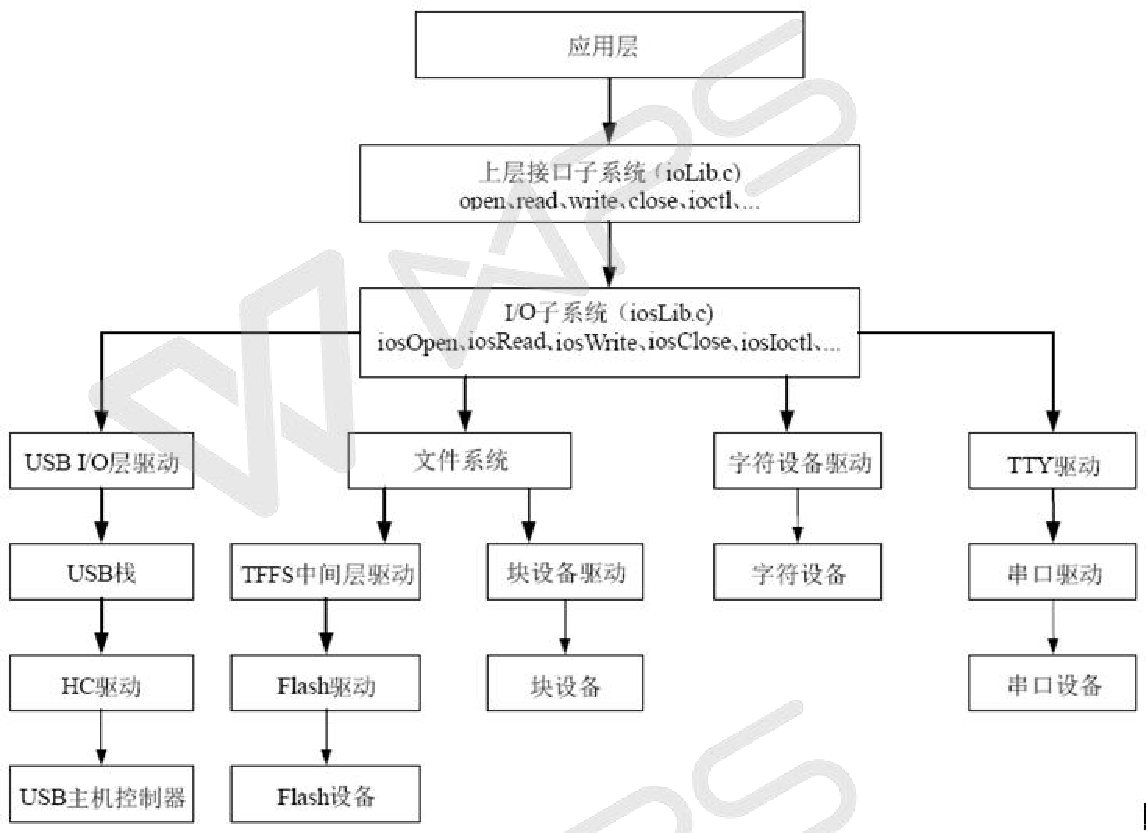
\includegraphics[width=\textwidth]{./graphics/VxWorks-driver-structure.pdf}
  \caption{VxWorks-driver-structure}
  \end{subfigure}
  ~
  \begin{subfigure}[b]{0.3\textwidth}
  \includegraphics[width=\textwidth]{}
  \caption{图片2}\label{fig:2-2}
  \end{subfigure}
\caption{多个图片}\label{fig:2}
\end{figure}

\section{参考文献示例}
这是一篇中文参考文献\cite{徐媛媛2003嵌入式实时操作系统的设备驱动};这是一篇英文参考文献\cite{9787508342894};同时引用\cite{9780124467422,bamboosilk}。

\section[\textbackslash{}autoref 测试]{\texttt{\textbackslash{}autoref} 测试}

\begin{description}
  \item[公式] \autoref{eq:1}
  \item[脚注] \autoref{footnote:1}
  \item[项] \autoref{item:1},\autoref{item:2},\autoref{item:3}
  \item[图] \autoref{fig:1}
  \item[表] \autoref{tab:1}
  \item[附录] \autoref{appendix:1}
  \item[章] \autoref{chapter:1}
  \item[小节] \autoref{sec:1},\autoref{sec:2},\autoref{sec:3}
  \item[算法] \autoref{alg:1},\autoref{alg_line:1}
  \item[证明环境] \autoref{def:1},\autoref{proposition:1},\autoref{axiom:1},\autoref{lemma:1},\autoref{theorem:1},\autoref{proof:1}
\end{description}}